\documentclass[a4paper]{article}

% CJK support: prefer ctex, fallback to XeTeX native line breaking
\IfFileExists{ctex.sty}{
  \usepackage[fontset=fandol]{ctex}
}{
  % Fallback for minimal TeX installs (e.g. MacTeX Basic, TeX Live scheme-basic)
  % without ctex/xeCJK. Uses XeTeX's built-in CJK line breaking.
  \usepackage{fontspec}
  \XeTeXlinebreaklocale "zh"
  \XeTeXlinebreakskip = 0pt plus 1pt
  \IfFontExistsTF{Songti SC}{\setmainfont{Songti SC}}{%
    \IfFontExistsTF{Noto Serif CJK SC}{\setmainfont{Noto Serif CJK SC}}{}%
  }
  \IfFontExistsTF{Heiti SC}{\setsansfont{Heiti SC}}{%
    \IfFontExistsTF{Noto Sans CJK SC}{\setsansfont{Noto Sans CJK SC}}{}%
  }
}

% Basic packages
\usepackage{amsmath, amssymb}
\usepackage{graphicx}
\usepackage[margin=2.5cm]{geometry}
\emergencystretch=3em
\usepackage[most]{tcolorbox}
\usepackage{etoolbox}
\usepackage{listings}
\usepackage{hyperref}
\usepackage{booktabs}
\usepackage{array}
\usepackage{subcaption}
\usepackage{float}
\usepackage{tikz}
\IfFileExists{pgfplots.sty}{
    \usepackage{pgfplots}
    \pgfplotsset{compat=1.18}
}{}

% ===== Highlight boxes =====
\newtcolorbox{knowledgebox}[1]{
    enhanced, colback=blue!5!white, colframe=blue!75!black, colbacktitle=blue!75!black,
    coltitle=white, fonttitle=\bfseries, title={#1}, attach boxed title to top left={yshift=-2mm, xshift=2mm},
    boxrule=1pt, sharp corners
}

\newtcolorbox{importantbox}[1]{
    enhanced, colback=yellow!10!white, colframe=yellow!80!black, colbacktitle=yellow!80!black,
    coltitle=black, fonttitle=\bfseries, title={#1}, sharp corners
}

\newtcolorbox{warningbox}[1]{
    enhanced, colback=red!5!white, colframe=red!75!black, colbacktitle=red!75!black,
    coltitle=white, fonttitle=\bfseries, title={#1}, sharp corners
}

\newtcolorbox{practicebox}[1]{
    enhanced, colback=black!3!white, colframe=black!75, colbacktitle=black!75,
    coltitle=white, fonttitle=\bfseries, title={#1}, sharp corners
}

% ===== Code listings =====
\lstset{
    basicstyle=\ttfamily\small,
    keywordstyle=\color{blue},
    stringstyle=\color{red!60!black},
    commentstyle=\color{green!60!black},
    breaklines=true,
    frame=single,
    numbers=left,
    numberstyle=\tiny\color{gray},
    captionpos=b,
    extendedchars=false
}

% ===== Figure provenance and unit macros =====
% \vtag goes inside \caption{...}; \srcnote{MM:SS--MM:SS} follows the figure environment.
\newcommand{\vtag}{\protect\footnotemark}
\newcommand{\srcnote}[1]{\footnotetext{视频画面时间区间：#1。若为裁剪图，时间区间仍对应原视频画面。}}
% Units work in text and math mode; never hand-write $^\circ$ or \AA inside \mathrm.
\newcommand{\degC}{\ensuremath{^{\circ}\mathrm{C}}}
\newcommand{\um}{\ensuremath{\mu\mathrm{m}}}
\newcommand{\nm}{\ensuremath{\mathrm{nm}}}
\newcommand{\angstrom}{\ensuremath{\text{\AA}}}

% ===== Front-page metadata =====
% Fill these in when generating notes.
\newcommand{\notetitle}{代码之外}
\newcommand{\notesubtitle}{MIT Missing Semester 2026 · 第 8 讲：注释、提交信息、bug 报告、拉取请求、代码评审、提问与 AI 礼仪}
\newcommand{\noteauthors}{根据 MIT Missing Semester 2026 课堂录像整理（Jon 主讲）}
\newcommand{\notedate}{2026年1月22日（课堂）}
\newcommand{\videochannel}{Missing Semester（YouTube）}
\newcommand{\videopublishdate}{2026年}
\newcommand{\videoduration}{1小时5分37秒}
\newcommand{\videourl}{https://www.youtube.com/watch?v=2DOEATfXT8k}
\newcommand{\videocoverpath}{cover.jpg}

\setlength{\emergencystretch}{3em}
\begin{document}

% ===== Title page =====
\begin{titlepage}
\centering
{\Large 课程笔记\par}
\vspace{1.2cm}
{\huge\bfseries \notetitle\par}
\ifdefempty{\notesubtitle}{}{
\vspace{0.3cm}
{\large \notesubtitle\par}
}
\vspace{0.5cm}
{\large \noteauthors\par}
\vspace{0.3cm}
{\large \notedate\par}
\vspace{1.0cm}

\ifdefempty{\videocoverpath}{
{\small 请在生成笔记时填入视频封面图的本地路径。\par}
}{
\includegraphics[width=0.82\textwidth,height=0.40\textheight,keepaspectratio]{\videocoverpath}\par
}

\vfill
\begin{tcolorbox}[width=0.9\textwidth, colback=black!2!white, colframe=black!60, sharp corners]
\textbf{视频作者/频道}：\videochannel\par
\textbf{发布日期}：\videopublishdate\par
\textbf{视频时长}：\videoduration\par
\textbf{视频链接}：
\ifdefempty{\videourl}{
未填写
}{
\href{\videourl}{\nolinkurl{\videourl}}
}
\end{tcolorbox}
\end{titlepage}

\tableofcontents
\newpage

%% --- 正文内容开始 --- %%

\section{这一讲讲什么}

\noindent\begin{minipage}{\textwidth}
\begin{figure}[H]
\centering
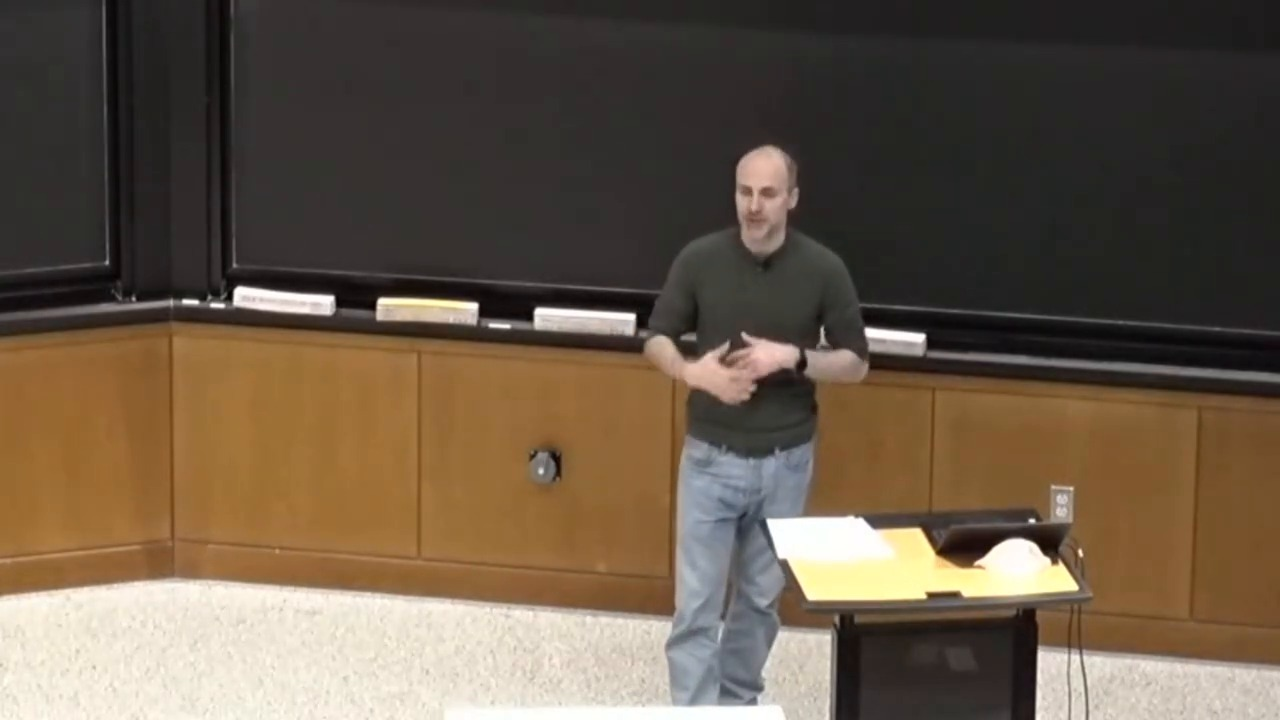
\includegraphics[width=0.92\textwidth]{figures/fig_01_room.jpg}
\caption{第八讲没有幻灯片，讲者 Jon 直接面对听众讲述工程师的协作\vtag}
\end{figure}
\srcnote{00:00:30--00:00:45}
\end{minipage}


讲者 Jon 开场就说，这一讲的内容感觉和代码没什么关系，和工程、和电脑的技术方面也没什么关系，讲的是围绕“做一名工程师”的软技能。而这恰恰是他认识的大多数工程师最吃力的地方之一：他们技术上往往很强，难的是与他人协作，知道怎样与在线生态互动，怎样与其他工程师、与项目维护者打交道。这一讲他不会在黑板上写东西，只是讲讲做工程师是什么样子，以及应该怎样看待与其他工程师的互动。

\begin{importantbox}{一半是代码，一半是沟通}
讲者认为，做一名好的软件工程师，大约 50\% 在于写好的代码、构建好的系统，另外 50\% 在于与他人沟通：告诉别人你的系统怎样工作，帮他们上手；也从他们那里了解他们需要你的系统做什么；与那些系统要和你的系统交互的工程师打交道；与用户互动等等。
\end{importantbox}

\begin{knowledgebox}{本讲结构}
讲义作者整理：讲者把这一讲分为四部分。单向沟通，包括代码注释、README 和提交信息；双向协作，包括提交 bug 报告、拉取请求以及代码评审；教育，即怎样提问；最后是使用 AI 的礼仪。
\end{knowledgebox}

\section{单向沟通：代码注释}

讲者说，单向沟通是你写东西给其他工程师看，不是对话，不是打视频电话，而是你把东西写下来，他们在将来某个时候、可能与你相隔很远的情况下去处理。最主要的载体就是代码注释：写注释是你与将来查看同一份代码的工程师交流的主要方式之一，而那个人也可能是六个月或一年后的你自己，那时你已经记不得写代码时脑子里的那些东西了。

\subsection{不要只解释代码做了什么}

讲者觉得代码注释往往没有被有效使用：大家知道应该写注释，却不知道该写什么。他见得最多的注释是解释代码做了什么的，而这也是最没用的注释，因为代码就在那里，读代码就知道它做什么。真正值得写进注释的，是那些不容易从代码中解析出来的东西，这样用的注释价值极高。

\subsection{值得写的几类注释}

\begin{itemize}
\item 待办（TODO）：在代码里写 \texttt{// TODO:} 加上描述，说明代码库中这个位置附近需要修改的地方。也可以用问题跟踪系统，但有时直接写在代码里很有用，别人以后很容易找到，比如用第一讲介绍的 \texttt{grep}。
\item 出处（references）：在有些代码库中更常见，你会实现来自别处的算法：可能是用另一种语言实现过、你移植过来的；可能来自论文或博客文章；也可能是某门课或某本教科书里的数据结构。放一个出处链接对后来的人极其有用：否则他们只看到一串奇怪的代码，最终发现它是在给数组排序；有了出处，他们就知道这个函数是用来排序的，也知道为什么这个算法这样工作、你为什么选择它。
\item “为什么不”（why nots）：讲者特别推荐这一类，用注释解释你为什么没有用显而易见的方式去做。
\end{itemize}

讲者解释“为什么不”：也许你按直接的方式写了代码，结果不行，花了两个小时调试。比如显而易见的做法是用编程语言标准库里内置的字典或哈希表类型，但由于某种原因，对这段代码来说那是个坏主意，所以你用了别的数据结构，它实际上也是一个映射，你也把它当映射用，只是没用标准库的那个。为什么？你需要在注释里解释为什么做出了不同于默认的选择。否则以后会有某个聪明的工程师读到这段代码，心想“这不就是个映射吗，换成标准库的吧”，然后重新经历一遍你经历过的痛苦，才发现那样为什么不行。你当时做出选择时的洞见，否则就会随时间流失。

\begin{lstlisting}[language=Python]
# TODO: retry with exponential backoff once the API supports it.

# Implements the algorithm from Section 3 of
# "Some Paper Title" (https://example.org/paper.pdf).

# Why not dict? Keys arrive in insertion order and we need O(1)
# eviction of the oldest entry; see issue #123 for the benchmarks.
\end{lstlisting}

\begin{warningbox}{示例说明}
讲义作者提醒：上面三条注释是讲义作者为说明三类注释而编写的示例，其中的论文标题和问题编号均为虚构的占位符。
\end{warningbox}

讲者说还有其他几类，讲义里也列了一些。

\section{单向沟通：README 与提交信息}

\subsection{README 的顺序}

第二种单向写作是 README。讲者认为好的 README 应该按顺序回答几个问题：
\begin{enumerate}
\item 这是什么？不要假设来到你仓库的人已经知道这个项目是什么。
\item 我为什么要关心？比如有人只是在四处找有趣的项目来贡献，看到描述后可能会想“我不需要这个”；要说明它做什么、为什么有意思、为什么不平凡。
\item 怎样使用？假设读者根据前两点认定它有用、也明白它做什么，现在想用它，怎样开始？
\item 怎样安装？现在知道怎样用、也决定要用了，怎样装到自己电脑上？
\end{enumerate}

讲者强调顺序很重要：很多项目的 README 一上来就是安装说明，可我还没决定要不要用，为什么先给我安装说明？然后还有一堆基本没用的东西，他都懒得逐一讲，因为放在那里没有意义。总的来说，README 要保持相当简洁，让人能把它当作可以快速浏览的有用参考。

项目里通常还有其他文件解释项目的其他方面。比如有的项目有 \texttt{CONTRIBUTING.md}，说明想为项目做贡献时流程是怎样的：提交 bug 报告和拉取请求（即对项目的修改）的流程、怎样测试、代码中你可能不习惯的约定等等。这些不必放进 README，可以放在单独的文件里，因为 README 面向的是使用者，而 CONTRIBUTING 面向的是协作者。

\begin{practicebox}{检查一个 README}
讲义作者整理：找一个你常用的开源项目，看它的 README 是否依次回答了“是什么、为什么关心、怎样用、怎样装”；如果没有，试着按这个顺序重写开头的几段，并把面向贡献者的内容移到 CONTRIBUTING.md 中。
\end{practicebox}

\subsection{提交信息：写“为什么”}

第三种单向写作是提交信息。讲者说版本控制那一讲已经讲了很多 Git，但没有讲 Git 卫生（Git hygiene）：不是命令行意义上，而是与他人协作意义上应该怎样使用 Git。Git 提交不仅让你说“这是一堆修改，替我存起来”，还让你对这些修改做额外的说明。这里同样容易落入陷阱：在提交信息里只写修改了什么。

但修改了什么通常从修改内容本身就能看出来：运行 \texttt{git diff}，看到这里被改成了那样，就知道改了什么。人们想知道的是：你为什么做这个修改，为什么用这种方式做。提交信息是一份历史记录，说明代码库为什么以这种方式而不是别的方式演化。有一个工具叫 \texttt{git blame}：指向 Git 仓库中的一个文件，它会告诉你每一行最后是被哪个提交修改的，你可以去看那个提交的信息，看这一行为什么改、改之前是什么样，还可以一直沿着历史往回追。但这类工具只有在提交信息真正解释了“为什么”时才有用。

\begin{importantbox}{提交信息应回答的问题}
讲者列出提交信息通常应该回答的几点，并说明有些在显而易见时可以省略：
\begin{itemize}
\item 是什么问题迫使你做这个修改？为什么这个修改是必要的？
\item 你考虑过哪些替代方案？为什么不用别的方式？如果只是修一个差一错误，没有真正的替代方案，这一项就不需要。
\item 这个修改有什么权衡或影响？
\end{itemize}
\end{importantbox}

讲者解释权衡：有时你的修改有望让事情变好，但也可能让某些事情变差。优化尤其常见：你做了基准测试，发现常见情况下变快了，但有些情况变慢了，因为真正免费的优化很少见。所以要解释为什么做出这个权衡，为什么你认为好处值得代价。同样要指出不明显的影响：比如在构建过程和运行时分开的语言中（Python 不是这样，但 C、Rust 等编译型语言是），如果你的修改让程序运行更快、却让项目构建更慢，这就值得写进提交信息，因为这是你选择的一个权衡，而只看差异的人并不能看出来。评审你的修改的人可能不同意这个权衡，这些额外的上下文对他们非常有用。当然，细节的多少应该与复杂度相称：修改越大越复杂，给的上下文越多；微不足道的修改，可以少给很多。讲者说，现在看起来显而易见的东西，一两年后就不再显而易见了。

\subsection{用 LLM 写提交信息}

讲者说 LLM 在写好的提交信息方面其实很有帮助。问题在于：如果直接让 LLM 帮你写提交信息，它会吐出一大段关于“改了什么”的各种细节。因为归根结底，你把差异给它、让它写提交信息，它唯一的上下文就是差异，也就是改了什么；它不知道为什么，不知道权衡和影响。所以用 LLM 写提交信息时，通常采取两种做法之一：

\begin{itemize}
\item 如果你本来就用 LLM 做了这个修改，就在同一个会话里让它写提交信息。因为你在提示它修改代码时进行的那段对话给了它上下文，对话本身就是上下文，这时它对“改了什么、为什么、有什么影响”知道得多得多。
\item 在提示中告诉它：如果你发现某些东西不明显、不理解为什么做这个修改，就来问我。于是这变成一个交互式会话，LLM 基本上把你当作“神谕”、当作一个可以查询额外信息的智能体工具，来写出更好的提交信息。
\end{itemize}

但它默认不会这样做，你必须确保它既理解你想在提交信息里放什么，又在过程中收集到这些信息；否则它只会产出一段看起来很厉害、却只是复述差异的提交信息。

\subsection{把修改拆成有意义的提交}

讲者说另一个常见问题是：你做了一堆修改，\texttt{git add .} 加上所有东西，\texttt{git commit}，写个提交信息就推上去了。这对别人回顾历史或评审都不太有用，因为它是一个巨大的修改，可能包含很多互不相关的改动。最明显的例子是你还对代码运行了格式化工具，于是差异巨大，但大部分只是格式变化，只有一部分是语义变化。所以一般应该把逻辑上或语义上独立的修改分到不同的提交里。

做法是 \texttt{git add -p}：它会逐块显示当前差异，问你“要把这一块加入即将进行的提交吗？”，你回答是或否。这样就能从当前差异中有选择地把内容加入暂存区，提交，再 \texttt{git add -p} 加入其他修改，如此推进。LLM 在这里也能帮忙：可以告诉它“我有一堆差异，找出语义上相关的部分，尝试为它们分别写提交”，事后你可能需要清理一下，也要确保它拿到上下文，但它是把巨大差异拆分成逻辑上独立的提交的有用工具。

\begin{lstlisting}[language=bash]
git add -p          # stage hunks one at a time
git commit          # commit the first logical change
git add -p          # stage the next group of hunks
git commit
\end{lstlisting}

有了多个提交，还可以为评审开多个彼此独立的拉取请求，这在开源项目中尤其有用。讲者说，如果你给开源项目带去一个包含多个不相关修改的巨大差异，他们会让你走开，带着结构更好的拉取请求再来；他们不会评审包含大量无关修改的东西。部分原因是他们可能想接受一部分修改、拒绝另一部分：也许不要你的格式化修改，但很想要你的新功能。如果拆成多个拉取请求，他们就可以在有时间时一块块评审，先合并没有争议的，把需要更多讨论的留着。这样你的修改能更快进入项目，待评审的东西也会随时间减少。

\subsection{尊重读者的时间}

讲者也提醒了一句：当你开始努力做好技术写作，无论是注释、提交、README 还是别的地方，都有钟摆摆得太远、开始写得太多的危险。写任何沟通内容时，尊重读者的时间非常重要。读者最终会发现文字太多，于是一个字都不读。没有文字，当然没人读；文字很少，他们会读；而在某个临界点，他们会想“我才懒得看”，或者读完第一段就停了。所以写给其他工程师看的东西时，想想如果你是那个读者，会不会愿意读。用 LLM 写东西时尤其如此，因为 LLM 非常擅长生成大量文字，你通常需要非常具体地要求它：给出简洁的总结，而不是长篇大论。

\subsection{git bisect 与好的提交}

讲者补充了一个说明好提交信息为什么有用的例子：\texttt{git bisect}。假设你在某个开源软件里发现一个 bug，而它以前没有，你更新软件后才出现。\texttt{git bisect} 让你说：这是软件正常工作的版本，这是不正常的版本，帮我找出引入问题的提交。它用二分法，也就是二分查找：先检出中间的提交，让你判断是好是坏，然后在对应的一半里继续二分，直到找到引入 bug 的那个提交。但如果那个提交没什么用，比如提交信息完全没解释为什么从 A 改成 B，或者差异里改了很多不相关的东西，那二分对你弄清是什么引入了 bug 就帮助不大，你还得做更多调试。

\texttt{git bisect} 也可以自动化：如果能用测试复现 bug，就可以给 \texttt{git bisect run} 传一个脚本，它根据 bug 是否存在以成功或失败退出，Git 会自动完成整个二分过程。

\begin{lstlisting}[language=bash]
git bisect start
git bisect bad                 # the current version has the bug
git bisect good v1.2.0         # this older version worked
git bisect run ./test_bug.sh   # exit 0 = good, non-zero = bad
git bisect reset
\end{lstlisting}

\begin{knowledgebox}{二分查找需要多少步}
讲义作者补充：二分查找每一步把候选范围减半，所以在 $n$ 个提交中定位引入 bug 的那个，大约只需要 $\log_2 n$ 次测试。例如在 1000 个提交之间，大约 10 次测试就够了。前提是每个提交都能独立构建和测试，这又一次说明了保持提交小而完整的价值。
\end{knowledgebox}

\section{双向协作：bug 报告}

\subsection{维护者的时间极其有限}

讲者说，最常见的协作方式也许是贡献：你向别人提交修改或 bug 报告，而他们是项目的权威。对 bug 报告来说，对方可能是项目维护者；对拉取请求来说，可能是一位资深工程师会评审你的修改，告诉你在合入代码库之前要改什么。无论提交什么，都要记住：用户和维护者在数量上相差一个数量级甚至更多。这对开源项目尤其是个现实问题：可能有上百万用户，却只有两个甚至一个维护者，他们的时间严重超额。

因此你要花额外的力气，确保提交给他们的东西已经处于值得他们花时间看的状态。部分原因是尊重他们的时间，另一部分是出于自身利益：如果 issue 或拉取请求不规范，他们会忽略它。如果他们认为不值得花时间，可能直接关掉 issue 或置之不理；拉取请求可能永远不被评审，或者搁置一年，等他们有更多时间再说，而我们都知道，人永远不会有更多时间。

\subsection{好的 bug 报告的要素}

讲者说提交好的 bug 报告是一种会随时间进步的技能，但只有你去尝试、真正练习才会进步。他列出好的 bug 报告的几个基石：
\begin{itemize}
\item 带上足够的上下文，让别人能复现问题：通常包括你所处的环境，比如操作系统、软件的版本号、你的配置文件等。
\item 你期望看到什么，以及实际发生了什么：好的 bug 报告显然要说出了什么问题，但也要说你期望发生什么。因为有时你观察到的其实就是预期行为，只是与你的预期不符；那不一定是软件的 bug，可能是文档的 bug，文档本应更好地向你说明软件是这样工作的。这个差别对查看报告的维护者很有用。
\item 复现步骤：讲者说这也许是最重要的，通常是一个有序的编号列表：打开程序，做这件事，点这里，在这里输入这个，按回车，然后我期望发生的没有发生，而是发生了这个。
\item 你已经尝试过什么：为了绕过这个 bug 试过哪些办法，或者看过代码、试着弄清哪里出了问题。让他们看到你也付出了努力。即使没时间自己深入代码，提交 bug 报告仍然有用；但如果能做，会非常有帮助。
\end{itemize}

\subsection{最小可复现示例}

讲者说，提交 bug 报告时最好的做法之一，是提供一个可复现的示例。有时就是复现步骤；如果你依赖某个代码项目，比如一个代码库，复现示例往往是你给他们的代码：我这样用你们的库，它就不能正确工作。如果你只给一个巨大项目的链接，说“我编译它时不对”，对维护者完全没用：如果你有一个 100,000 行的代码库，碰巧用了他们的项目，然后说“我的东西不工作”，他们会忽略你。你要做的是制作一个最小可复现示例（minimal reproducing example）：从你手头的软件开始，尽可能多地砍掉东西，只留下用这个软件触发 bug 所必需的部分。

讲者承认这可能要做很多工作，但这本来就是维护者为了修你的 bug 必须做的工作：只有他们自己能复现，才能修。所以要么你花时间做出复现，要么他们得找时间做；而通常最好是你来做，如果你能做的话。

\begin{practicebox}{制作最小复现}
讲义作者整理：遇到一个疑似库的 bug 时，新建一个空目录，只安装出问题的那个库（固定版本），写一个尽可能短的脚本触发问题；然后逐行删除代码、逐个去掉参数，每删一步都确认问题仍然存在，直到再删任何东西问题就消失为止。把这个脚本、库版本、操作系统和完整的错误输出一起放进 bug 报告。
\end{practicebox}

\subsection{先搜索，不要只说“我也是”}

另一个常见的失败模式，尤其是向开源仓库提交 bug 报告时，是不先搜索是否已经有人报告过同样的问题。重复报告极其常见，而且与用户的技术水平负相关：用户越不懂技术，提交重复报告的越多，留下“我也是”“+1”这种评论的也越多。讲者说这些都是噪音，而且噪音有双重坏处：一方面让其他人更难找到是否已有类似的问题，因为要搜的东西多了很多；另一方面维护者要从噪音中筛出真正的信号，痛苦得多。

还有第三个坏处：假设你用的某个开源软件有个 bug，你很想知道它什么时候修好，于是订阅了那个 issue，通过 GitHub 通知或者邮件。现在几百个人在下面评论“我也有这个问题”“为什么还没修”“这个 bug 都开了两年了”，这些评论会发给每一个关心这个 bug 的人，纯粹是噪音，毫无价值，维护者早就知道有问题，因为 issue 就在那里。讲者说，在 GitHub issue 上，最接近有用的做法是给最上面那条帖子点个大拇指表情，维护者可以按这个给 issue 排序，这是“+1”唯一有用的形式。相反，如果你提供了“我做出了这个 bug 的最小可复现示例”或者“这是另一种复现方式，按这些步骤每次都能触发”，这些评论就极其有用，会大大增加 bug 被修好的可能。

\subsection{给维护者多一些宽容}

讲者提醒，维护者很多时候是志愿者，他们没有在你有空的时候有空，甚至可能几乎没有时间。所以当你想“这个 bug 怎么还没修”时要记住这一点。总体上要对开源维护者多一些宽容，因为他们负担太重。如果你提交了拉取请求，第二天就去催“能帮忙评审一下吗”通常不值得；礼仪更像是：几周之后礼貌地跟进一下没问题。

他以自己为例：有人向他的仓库提交过拉取请求，他六个月都没时间看，他说这很糟，他也希望有时间，但就是没有。可能因为那是很久以前做的项目，他会轮流在不同项目上投入时间，而他如今花在开源上的有限时间，被他维护的其他开源仓库中更重要的 bug 占用了。这不是针对那位贡献者，只是开源生态依赖的是人们的志愿时间，与他们互动时要记住这一点。

有同学问什么是拉取请求：讲者解释，就是你向一个代码仓库提交修改：别人有一个仓库，你带着一个 Git 差异、一个或一组提交去找他们，说“能把这个合入你们的项目吗？”又有同学问有没有可以参考的好 bug 报告范例。讲者说并没有一个“去看这个就行”的标准范例，不过今天有一道习题就是让大家去找一些。之所以这样安排，是因为你往往很快就能看出一个 bug 报告或拉取请求是否有用，从维护者的回应方式也能看出来；提高的最好方式不是拿到一个管用的模板，而是观察这些互动，耳濡目染，看哪里有摩擦、哪里没有。有同学指出有些项目有自己的模板，讲者说：在 GitHub 上很多项目在你开 issue 或拉取请求时会自动填入一个模板，让你填写特定字段。这些模板在格式上有用，确保你按他们想要的格式写；但它们弥补不了对“什么是好的 bug 报告”缺乏理解，填空可以填得好也可以填得差，取决于你是否理解好的 bug 报告的目的：为维护者节省替你修复它的时间。

\section{双向协作：拉取请求与维护}

\subsection{提交拉取请求之前}

如果你决定开一个拉取请求，向项目提交修改，这就超出了提交 issue，而是真正贡献自己的修改。讲者提了几点：
\begin{itemize}
\item 先读 \texttt{CONTRIBUTING.md}，里面通常有额外的说明。
\item 看项目的许可证（license）：你向项目提交的修改通常会被纳入项目的许可证。比如项目以 GPL 授权，你的贡献合并后，那段代码就以与项目相同的 GPL 许可证发布，你不再对它有独占的控制，大多数其他常见许可证也是如此。通常这对你无所谓，但如果你是某公司的雇员，公司可能对员工能为哪些项目贡献有规定。所以在商业环境中工作时，要根据项目的许可证查清贡献政策。
\item 注意提交的卫生，拆分好提交，让每个拉取请求都能独立评审、单独有用。
\end{itemize}

\begin{warningbox}{关于版权的说法}
讲义作者提醒：讲者说贡献合并后“代码不再是你的、你没有版权”，这是口语化的简化。在许多项目中，贡献者保留自己代码的版权，只是按项目许可证授权；也有项目要求签署贡献者许可协议（CLA）把权利转让或授予项目方。具体以项目的 CONTRIBUTING 文件和许可证为准，在公司工作时还要遵守公司的开源政策。
\end{warningbox}

\subsection{一组必须一起接受的修改}

有时你有一系列修改，项目要么全部接受，要么全部不接受。比如为了实现一个功能，你必须修改项目中更底层的部分；但如果他们不要这个功能，也不应该接受这些底层修改。这时通常开一个拉取请求，说明“这个拉取请求包含两个提交，一个修改这部分，一个在它之上构建”，甚至可以给评审者指引：“建议逐个提交评审，而不是把整体差异当作一块来看。”讲者说维护者往往很欣赏这种评审指引，因为作为作者，你更清楚它应该怎样评审。

和提交信息一样，开拉取请求时通常要写描述。讲者说可以把它想成一封附带 Git 提交的邮件：你要在邮件里，或者说在 GitHub 的拉取请求里，说明为什么希望这个修改进入项目。这不只是“为什么用这种方式修改”，而是“为什么你认为项目应该有这个功能或这个修复”。

\subsection{接受修改意味着承担维护责任}

讲者解释了为什么维护者会犹豫：接受一个差异、把它合并进项目，意味着他们承担起对它的责任。如果他是某个项目的维护者，接受了你一个给项目增加 1000 行代码的差异，这 1000 行他就要永远维护下去；而作为贡献者，你不需要，你做完贡献可以一走了之，你得到了想要的功能，皆大欢喜。但维护者不仅要考虑这是不是想要的功能，还要考虑它的实现方式是否让他觉得能长期承担维护责任，以后加其他功能时不会与这个修改冲突。他需要在你的修改本身之外考虑所有这些。

\subsection{分叉}

还有另一个选择：如果你向项目贡献，维护者说不要这个修改，说超出范围、太大、不想要这个功能等等，你可以分叉（fork）：把现有项目复制一份，通常换个稍微不同的名字，然后由你发布和维护它，而他们继续单独维护原项目。讲者说分叉代价很高：现在有两个项目，各有一个维护者，功能和代码大量重叠，维护者的时间被分摊到同一个代码库的两个副本上；一个收到改进的拉取请求，另一个并不会得到改进。

所以应该有非常非常好的理由才说“这需要分叉”：比如原项目的范围与你的目标不同，这会是一个实质上不同的项目，而这个功能对它很重要。如果只是“我的功能没被接受”，那通常不是分叉的好理由，而且你会对结果不满意：你会成为这个软件（或者说这个副本）唯一的维护者，只要你还在用，就得永远自己维护。你会定期去看原项目有哪些变化、确保能合并到你的项目、定期测试、做评审、接受贡献、处理别人提交的 bug 报告吗？

\subsection{成为维护者}

有同学问：有没有人主动提出成为自己贡献的那部分的维护者？讲者说要看项目规模。比如 Linux 内核有很多子系统，不同子系统有不同的维护者，部分就是这个原因：某个子系统的维护者是真正深切关心它的人，因为他们用它，或者写了大量代码等等。所以如果有人带来一个全新的子系统，几乎会有一种期待：至少你应该愿意长期维护它。小项目中这不太常见，原因之一是它行不通：一个 2000 行的项目，有人说“我来维护这 50 行”，那没什么意义，因为代码库随时间变化时，修改往往扩散到整个代码库，功能并不是一块永远不会再变的连续代码，只维护一部分的人往往会忽略整体；而且多个维护者有很多协调开销，除非能换来很多好处，比如一位完整的新维护者，项目通常不想要。

不过，为开源项目做贡献往往是你自己走向维护者的最好起点。成为开源项目维护者的，通常是贡献最多的人；最终也许维护者会说“我没时间了”，然后把项目交给你。但只有长期证明自己是值得信赖的、可靠的好贡献者，你才会得到这样的机会。

\subsection{AI 生成的拉取请求}

讲者说，AI 当然也进入了这个领域。做这一讲的习题、探索开源项目时你会看到，如今有大量由 LLM 生成的拉取请求，有些有用，大多数没用。原因是让 LLM 替自己提交拉取请求的人往往不充当过滤器，只是说“我想实现这个功能，做个提交，开个拉取请求”，结果通常结构不佳：不够精简，夹带一堆与修改无关的东西，描述又长又空。当维护者问“你为什么改这个？为什么这里必须改？为什么不改那里？”时，必须回复评论的人类作者往往答不上来，因为修改不是他做的，他不知道它为什么选择 A 而不是 B，他只是把修改的生产自动化了。所以开源维护者常常对 AI 写的拉取请求相当怀疑。

\begin{importantbox}{用 AI 贡献时你必须在环中}
这不意味着你不能用 LLM 帮你做修改，恰恰相反，它们可以很有用：写好的提交信息、写好的拉取请求描述，甚至处理评审意见。但你必须参与这个过程，确保自己理解为什么需要这个修改、为什么这样改。讲者说，如果你只是让 LLM 吐出一堆东西然后贴进拉取请求，维护者自己也完全可以这么做，而他们没做，很可能是有原因的。
\end{importantbox}

\section{代码评审}

\noindent\begin{minipage}{\textwidth}
\begin{figure}[H]
\centering
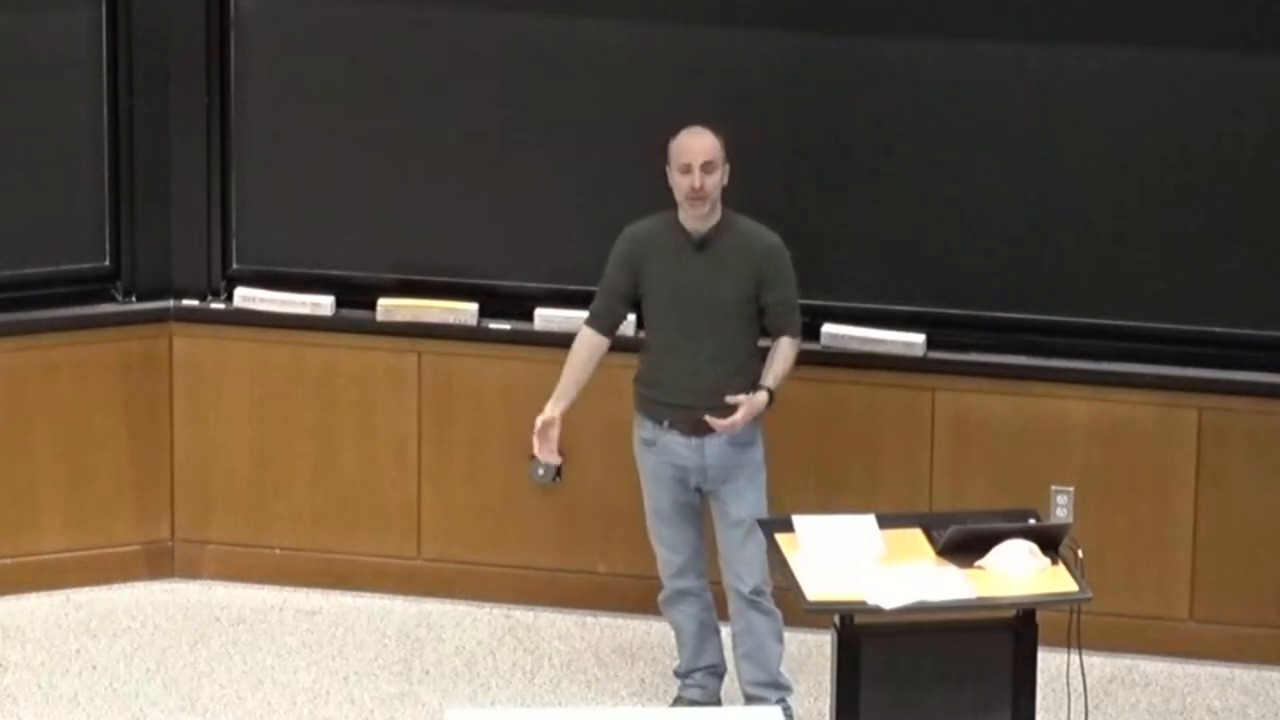
\includegraphics[width=0.92\textwidth]{figures/fig_02_room_review.jpg}
\caption{讲者谈代码评审：评审针对代码而非写代码的人\vtag}
\end{figure}
\srcnote{00:43:00--00:43:15}
\end{minipage}


\subsection{评审是关于代码的对话}

讲者说协作的下一步是评审。我们往往把代码评审想成：新手提交拉取请求，资深者评审，告诉他们哪里都错了。但评审其实只是一种异步讨论代码的方式：一个人提出修改，另一个人思考这个修改，然后一起讨论，几乎就像头脑风暴，看看什么好、什么不好。不幸的是，部分由于那种“资深者告诉你哪里写错了”的思维模式，评审形成了一种奇怪的语言，说“贬损”太重了，但确实让人感觉被评判，评审常常让人觉得“他们在告诉我我做错的每一件事”。讲者强调必须记住：代码评审不是关于写代码的人，而是关于代码本身，关于这段代码在这个项目中、为这个目的、在此时此刻是否合理。

他说你迟早会评审别人的代码，哪怕只是大学里的小组项目，你们也会、或者至少应该互相评审。部分原因是这是很好的学习方式：评审别人的代码既能发现错误，希望自己以后不犯，也能看到可以借鉴的好代码模式；还能读更多代码，了解更多概念。这是全面提升工程能力的好方法，会长期让你受益。

\subsection{好的评审意见}

除了记住评审的是代码而不是人，讲者还给了几条建议：

\begin{itemize}
\item 优先给可操作的意见。比如在 Python 或 JavaScript 中，文件顶部可以有全局变量，这通常是反模式，因为会让测试更难，比如不能并行运行两个测试，因为它们都读写同一个全局变量，会相互干扰。如果有人在你评审的拉取请求里用了全局变量，你可以在那一行评论“不要用全局变量”，但这不可操作：没告诉作者该怎么做，如果对方不知道这条建议，甚至没告诉他们错在哪里。更好的意见是：“能否把这些全局变量换成一个配置数据类？这样我们就能并行运行测试。”打字没多多少，帮助却大得多。
\item 提问而不是提要求。与其说“处理空值的情况”，不如说“如果这里传入空值会怎样？”意思一样，但一个语气更具协作性：一个是在评判人，“你怎么没想到这里可能是空值？”；另一个是“我读代码时想到，等等，这里是空值会怎样？”然后让对方自己意识到“对，那是错的，谢谢提醒”。讲者说这对贡献者的体验影响巨大，在开源项目中还会增加他们回来的机会，无论是处理你的评审意见，还是以后提交更多修改，甚至最终成为维护者；如果每次评审都让他们带着不快离开，他们就不会回来了。
\item 解释原因。说明你为什么认为某处不对，比如前面全局变量的例子，解释为什么不想用全局变量，为什么这个项目做了这个决定，因为对方可能没有这个背景。
\item 不要留太多意见。讲者说人们常犯的错误是留下远超必要的意见：如果评审有一百条意见，对方会一拖再拖，如果是工作，他们当然会处理，但仍会拖；他们也不知道哪些最重要；而且有时改了一处，其他几条意见就失效了，因为那段代码也得改。所以留一百条意见，往往只有五十条值得处理，另外五十条在前五十条处理完时已经无关了。同样，如果发现一个重复出现的模式，比如你希望变量以某种方式命名，在每个变量上都留一条意见只是噪音，不是信号，而且让人感觉你在痛打落水狗。
\item 区分阻塞和非阻塞的意见。讲者评审时，有些修改如果不做他就不会接受；有些是他更倾向这样做，但如果你更喜欢你的方式也行。区分这两类，对方就能分轻重缓急，先处理阻塞的，再进行下一轮评审，到时一些小问题可能已经不存在了。常见做法是在非阻塞意见前写 \texttt{nit:}，英语里 nit 指不太重要的小事。
\item 指出做得好的地方。讲者说这一点常被遗忘：评审者往往只关注必须改的东西，忘了指出别人做得很漂亮的地方。想象和人一起写代码，如果你每次开口都是说他做错了什么，那可不是什么愉快的体验，代码评审为什么要不一样？如果发现对方做了一个很好的选择，就留言说出来。他们什么都不用做，点“已解决”就行，但会让他们的一天好一点，也让评审更平衡，他们离开时对自己的贡献感觉更好，也更有动力去做你要求的修改。
\end{itemize}

\begin{lstlisting}[language=bash]
Not actionable:   Don't use globals.
Actionable:       Could you replace these globals with a config dataclass?
                  That way we can run the tests in parallel.

Demand:           Handle the null case.
Question:         What happens if null is passed here?

Non-blocking:     nit: maybe call this `retry_count` for consistency?
\end{lstlisting}

\subsection{AI 评审的局限}

讲者说，如今很多人用 AI 工具做评审，效果可以很好，他不是说不行，但它无法真正替代人类评审。原因之一是，至少目前，AI 评审只根据修改的描述和差异来评审。而实际评审代码时，大多数意见其实并不关于差异本身，当然会有一些，但评审真正存在的意义、更重要的意见，是看这个修改对整个代码库是否是个好主意，是否符合你在构建的产品或应用的方向，这个库是否应该这样变化，这个修改是否与版本方案不兼容、而你还没准备好发布一个破坏性版本。这些 AI 评审者没有上下文。所以 AI 代码评审是有用的工具，但不要以为它满意了，维护者也会满意。

有同学问能否在 AI 评审之前给它喂上下文。讲者说在一定程度上可以，但按他的经验，这正是触及 AI 能力边界的地方：很多事情它并不理解问题本身，你可以给它大量关于破坏性变更的上下文，但它不一定理解什么是破坏性变更，能用英语在句法上复述出来，但那更像模式重复，而不是理解这个项目的破坏性变更政策。有同学问 AI 会不会发展到能做到这些，讲者说这就涉及他是否认为当前的 AI 路线通往 AGI，他并不这么认为，但那是可以另外讨论的话题；它们可以非常有用，但他不认为只是给它们更多上下文的问题。

\section{教育：怎样提问}

讲者说讲完了单向沟通和双向沟通，现在讲教育。作为工程师，我们很多非写代码的时间其实花在向别人提问或回答别人的问题上：可能是导师、老师、助教，也可能是懂得我们不懂的东西、或者已经做完实验而我们还没做完的同学。无论是学还是教，这都是值得提高、也确实可以提高的东西。他特别希望更多人学会更好地提问；学会更好地回答问题往往是第二阶段，第一阶段是怎样提出能得到有用答案的好问题。讲义里链接了 Julia Evans 的一篇很好的博客文章，他强烈推荐阅读，并给出了一个简要总结：

\begin{itemize}
\item 先陈述你的理解：告诉对方“这些是我已经弄清楚的、我想过的、我知道的”，然后再提问，这样他们知道哪些不用重复。
\item 问是非题：这也许有点反直觉，我们往往觉得应该问个问题，让对方把所有细节讲出来；但有时更有用的是有针对性地试探，这样不会陷入你不关心或与问题无关的长篇离题。问是非题，你会很快弄清哪些理解对了、哪些没对；所以要在是非题里放尽可能多的细节，让对方要么能清楚地回答是或否，要么能从你的问题中看出你误解了什么并指出来。
\item 明确承认你不懂的地方：如果提问时假装自己懂，就得不到有用的答案，因为对方无法校准你在各个知识点上处于什么水平；你提问的全部原因就是想懂得更多。
\item 不要接受不完整的答案：讲者常看到有人提问后得到一个答案，因为不想再麻烦对方，虽然没听懂，还是说“好的谢谢”就走了。不要这样，因为你什么也没学到。要训练自己在真正理解之前不接受答案，或者直到明显该告辞为止。
\item 先自己做些研究：如果你提问前完全没有自己思考、搜索，对方如果是好人可能还是会帮你，但会有点恼火你连最起码的功课都没做。有时问题有显而易见的答案，搜一下或问 LLM 三秒钟就有了，那比让所有人都来问同一个答案很容易找到的问题要好得多。
\end{itemize}

讲者说，这些同样适用于问 LLM：给出具体的问题，说明你知道什么，不要因为它给了一个答案就罢休，用是非题去追问。也适用于在 Stack Overflow 等公共论坛提问：遵循这些指导，你会问出更好的问题，得到更好的答案，而之后有同样问题、找到你那个帖子的人也会从中学到更多，水涨船高。

\begin{practicebox}{改写一个问题}
讲义作者整理：把“我的程序报错了，怎么办？”改写成好问题：写明你想做什么、做了什么（附上最小复现和完整错误信息）、你目前的理解（“我认为是路径问题，因为……”），再提出一个具体的是非题（“是不是因为 \texttt{PATH} 中找不到这个命令？”）。
\end{practicebox}

\section{AI 礼仪}

讲者说最后讲 AI 礼仪，会很快。LLM 和 AI 在整个软件工程、乃至社会的很多方面越来越普及，而关于使用 AI 的社会和职业规范我们还没有弄清楚，它们仍在演变。昨天的智能体编程一讲已经讲了很多战术上的考虑，但还有一些更“软”的部分值得讨论。

\subsection{披露你使用了 AI}

讲者说，无论以什么形式用 AI 帮助你的工作，都需要披露。这不是关于羞耻，甚至不完全是关于学术诚信，更多是为了对你的产出设定预期，确保最终成果得到适当程度的审查。如果你没有披露用了 AI，而有很多代码你没真正读过、没仔细看过、不完全理解，那么别人知道这一点很重要，这样他们才知道在接受之前要对那部分额外审查。

他说用 LLM 本身没问题：他这几天一直在用 LLM 为工作上一个大项目写代码，那个任务非常适合 LLM，他对此毫无羞耻，因为这是合适的工具。但同样重要的是，最后交出这个生成的大代码库时，他要坦白“这些代码我没有全部读过，这是一个起点，我们之后会把它打磨成能在商业或生产中使用的东西”，起点需要明确标注为 AI 辅助的。而且最好说明哪些部分用了 AI、哪些没用：只说“这个项目用了 AI”对别人帮助不大，他们无法判断哪些该审查、哪些该怀疑、哪些该期待更高的质量标准。比如“我用 LLM 生成了这个项目的测试用例，但实际代码是我写的”，或者“我用它生成了 UI 前端，后端是我自己写的”，这些是需要坦白的有意义的区别。

\subsection{遵守团队和项目的规范}

你还要遵循所在团队、公司、项目的规范和期望。尤其在开源领域，商业环境中也一样，不同公司和项目有不同偏好，有时甚至有相当严格的规定，限定何时能用、何时不能用 AI，以及能用来做什么。有时理由很充分，比如“这里不能用 AI，因为那会违法”：公司不允许数据流出公司范围，而使用智能体 LLM 可能会把数据上传到公司无法控制的云服务。所以要留心，不要触犯法律；有时与法律无关，只是做一个尊重项目开发者意愿的贡献者。规范可能在光谱的任何一端，要熟悉你所在环境的偏好。

\subsection{你会学得更少}

讲者还提醒：用 AI 和 LLM 开发东西，你从过程中学到的会更少。自己动手做有巨大的学习成分，用智能体编程也能学到一些，确实能学到，但比自己写全部代码学得少。这是你做出的一个权衡：你想把时间花在哪里？有时你不想把时间花在写所有代码上，这没问题，有时你觉得那些代码本来也学不到多少东西。但这应该是一个有意识的选择、有意识的权衡。

\subsection{面试与考核}

最后，这也出现在面试和考核场合，无论是大学考试还是公司面试，越来越多的人想在这些场合以各种形式使用 AI。这里争议大得多：是否应该允许，是否可以，以及这是否意味着你评估的不再是人，而只是 LLM。同样要弄清考核场景设定了什么期望；如果不确定、也没有明确规定，就运用你最好的判断，并且最好去问一问。

\begin{warningbox}{不确定时就问}
讲义作者归纳讲者关于 AI 礼仪的要点：披露使用了 AI，并说明用在哪些部分；遵守课程、团队、公司和开源项目的规定，涉及数据外泄时尤其要小心；意识到用 AI 会少学一些，把它当作有意识的取舍；在考试和面试中先弄清规则，没有规则时主动询问。
\end{warningbox}

讲者最后提醒：明天的课前半部分讲代码质量，后半部分是答疑，讲义里有一个 Google 表单链接，请提前提交问题；明天照常 $1$:$30$ 上课，只有上周五因为 Mystery Hunt 改到了 3 点。

\section{总结}

\begin{itemize}
\item 工程师的工作一半是代码，一半是沟通。
\item 代码注释要写代码本身看不出来的东西：TODO、出处、“为什么不”。
\item README 依次回答是什么、为什么关心、怎样用、怎样装；面向贡献者的内容放进 CONTRIBUTING.md。
\item 提交信息写“为什么”：动机、替代方案、权衡与影响；用 \texttt{git add -p} 把修改拆成语义独立的提交；git blame 和 git bisect 依赖好的提交历史；尊重读者的时间，不要写太多。
\item bug 报告要有环境、期望与实际、复现步骤、已尝试的办法，最好附最小可复现示例；先搜索，不要只说“+1”；对志愿维护者保持耐心。
\item 拉取请求前读 CONTRIBUTING 和许可证，保持每个拉取请求独立可评审；合并意味着维护者承担长期责任；分叉代价高昂；用 AI 贡献时自己必须理解修改。
\item 代码评审针对代码而非人：给可操作的意见、多提问、解释原因、不要留太多意见、区分阻塞与 nit、指出做得好的地方；AI 评审缺乏项目上下文。
\item 提问时先陈述理解、问是非题、承认不懂、不接受不完整的答案、先自己研究。
\item 使用 AI 要披露、守规、有意识地取舍，在考核中先问清规则。
\end{itemize}

\begin{practicebox}{自测}
\begin{enumerate}
\item 为什么解释“代码做了什么”的注释最没用？举一个“为什么不”注释的例子。
\item 一条好的提交信息应该回答哪三个问题？为什么让 LLM 只看差异写出的提交信息往往不够好？
\item 为什么维护者宁愿收到三个小的拉取请求，而不是一个大的？
\item 把评审意见“这里要处理异常”改写成更好的形式。
\item 在什么情况下分叉一个项目是合理的？
\end{enumerate}
\end{practicebox}

\end{document}
